\section{Interfaz gráfica y Jugabilidad}

El juego como ya se ha comentado consistirá en ver cómo los NPCs aplican una estrategia concreta, en este caso es el jugador el que a través de botones puede interaccionar para cambiar la estrategia. En la siguiente figura podemos ver cómo queda la interfaz.

\begin{figure}[H]
    \centering
    \newcommand{\behaviourmodes}{../IA_Juegos/Assets/Textures/UI}
\begin{tikzpicture}
    \sffamily\sansmath
    \node[draw, rounded corners, minimum width = 5cm, minimum height = 1cm, fill = white] (0) {TOTAL WAR};
    \node (1) [right = -1.3cm of 0] {
\includegraphics[scale=0.11]{\behaviourmodes/AttackMode}};
    \node (2) [left = -1.3cm of 0] {
\includegraphics[scale=0.11]{\behaviourmodes/AttackMode}};
    
    \node[draw, align = left, rounded corners, minimum width = 1.5cm, minimum height = 1cm, fill = white] (3) at (-1.1, -1.1) {\phantom{l}A\phantom{llllllllllll}};
    \node (4) [right = -1.3cm of 3] {
\includegraphics[scale=0.11]{\behaviourmodes/AttackMode}};
    
    \node[draw, align = left, rounded corners, minimum width = 1.5cm, minimum height = 1cm, fill = white] (5) at (1.1, -1.1) {\phantom{l}A\phantom{llllllllllll}};
    \node (6) [right = -1.3cm of 5] {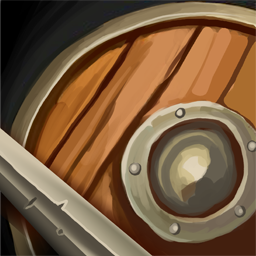
\includegraphics[scale=0.11]{\behaviourmodes/DefenseMode}};
    
    \node[draw, align = left, rounded corners, minimum width = 1.5cm, minimum height = 1cm, fill = white] (7) at (-1.1, -2.2) {\phantom{l}B\phantom{llllllllllll}};
    \node (8) [right = -1.3cm of 7] {
\includegraphics[scale=0.11]{\behaviourmodes/AttackMode}};
    
    \node[draw, align = left, rounded corners, minimum width = 1.5cm, minimum height = 1cm, fill = white] (9) at (1.1, -2.2) {\phantom{l}B\phantom{llllllllllll}};
    \node (10) [right = -1.3cm of 9] {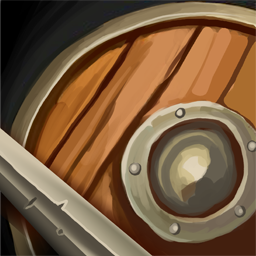
\includegraphics[scale=0.11]{\behaviourmodes/DefenseMode}};
\end{tikzpicture}
    \caption{Interfaz gráfica estrategia}
    \label{fig:mainButtons}
\end{figure}

Los iconos de espadas permitirán poner el modo ofensivo al equipo que se desee mientras que el icono del escudo permite indicar al equipo que se ponga a defender. El botón de \textit{Total War} cambia el comportamiento de todas las unidades del juego para que estas den prioridad al enfrentamiento y toma de la base rival. El juego comenzará con los botones desactivados.

Además tendremos una segunda UI a la que accederemos presionando la tecla \keys{I}. Esta nos permitirá tener el mapa de influencias en grande y el mapa de juego normal en un mini mapa, teniendo la siguiente interfaz que permite cambiar el mapa que se muestra \begin{figure}[H]
    \centering

    \begin{tikzpicture}
        \sffamily\sansmath
        \node[draw, rounded corners, minimum width = 5cm, minimum height = 1cm, fill = white] (0) {CAMBIAR MAPA};
        \node (1) [above = 0cm of 0] {MAPA ACTUAL: Tensión};
    \end{tikzpicture}
    \caption{Interfaz gráfica cambio de mapa}
    \label{fig:mainButtons}
\end{figure}
